\documentclass[Methods]{subfiles}
\begin{document}
\section{Methods}
\label{sec:Methods}

This section discusses the methods and tools that are used to measure the performance of Naxsi. Before both the approach and the methods are discussed in more depth, it is important to understand how the basic configuration looks like, which is discussed in the next section. Next, the tools that are used for measuring the performance and measuring the system resources, are briefly described. Lastly, the methods of the performance measurement are discussed.

\subsection{Experimental setup}
A configuration for standard web hosting that is seen quite often, is to separate the web hosting services on a functional basis. First, there is the web server, which is the front-end from a client's perspective. Second, there is the application layer. The application layer takes care of most of the processing power that is needed to process all the application logic. Third, there is the data layer, which is often a database server. It is not necessary to allocate these layers over different servers. Depending on the requirements, it is possible to host all services on one server. However, in order to do a performance measurement on one of these services, it is important that not all services run on the same server. Therefore, in this setup, every layer is taken care of by a dedicated server.

Figure~\ref{fig:Experimental setup} shows the setup that is used for the experiments. Table \ref{tab:Experimental infrastructure} gives a short description of each server and the service(s) that run(s) on it. Server01 is the front-end server, but it will also act as a software router for basic communication with the servers behind it. Server02 processes all the application data, which for a large part consists of the processing of PHP code. Server04 is used to execute the performance measurements. The hardware specifications and the software that is used, can be found in appendix \ref{sec:Experimental setup}.

\begin{figure}[H]
\caption{Experimental setup}
\centering
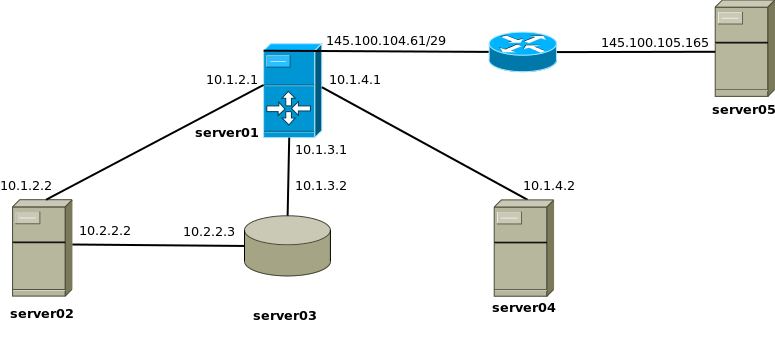
\includegraphics[scale=0.4] {images/infrastructure.png}
\label{fig:Experimental setup}
\end{figure}

\begin{table}[H]
\caption{Experimental infrstructure}
\begin{tabular}{|p{2,5cm}|p{3,5cm}|p{5cm}|}
\hline
\textbf{Hostname} & \textbf{Service} & \textbf{Short description} \\ \hline
server01 & Nginx + Naxsi & Front-end server and router \\ \hline
server02 & Nginx + Fastcgi & Application layer \\ \hline
server03 & MySQL & Data layer \\ \hline
server04 & Benchmark tools & Performance measurements \\ \hline
server05 & Collectd & Resource usage collector \\ \hline
\end{tabular}
\label{tab:Experimental infrastructure}
\end{table}

\subsection{Performance measurement tools}
A variety of performance measurement tools (also called benchmarking tools) exist. However, not all of them are suited to perform tests in this specific experimental setup. This section discusses a selection of the available tools.

\subsubsection{Apache Benchmark}
\emph{Apache Benchmark} is an open source web server benchmarking tool developed by Apache initially to test Apache web server installations.\footnote{\url{http://httpd.apache.org/docs/2.2/programs/ab.html}} However, it is not limited to Apache web servers, as it simulates regular HTTP requests.\\
During the execution of the performance tests, \emph{Apache Benchmark} is used when the number requests per second exceed the number of concurrent connections that are realistically possible. To be able to stepwise increase the number or URL parameters, as well as to calculate the avarage of repeated tests, a perl script is written to automate these operations~\footnote{\url{https://github.com/lutzengels/naxsiperftest/blob/master/tools/bench.pl}}.  These experiments are explained later in this section.


\subsubsection{Httperf/Autobench}
\emph{Httperf} is a web server performance measurement tool developed by David Mosberger~\cite{mosberger1998httperf} at Hewlet-Packard Research Labs~\cite{httperf}. It supports both HTTP/1.1 and SSL and aims to be robust enough to generate server overload. \emph{Autobench}~\cite{autobench2013} is a Perl script that wraps around \emph{Httperf}. It aims at automating the benchmarking process and offers extensive options, amongst which the ability to stepwise increase concurrent connections or the number of requests per second. 

In the course of this project, \emph{Autobench} is used to confirm and visualize the threshold of the number of concurrent connections that Naxsi can handle (as described in section~\ref{sec:Baseline performance measurement}). The automation of incrementing the URL parameters is done by wrapping a script~\footnote{\url{https://github.com/lutzengels/naxsiperftest/blob/master/tools/measure_naxsi_with_param_increments.pl}} around Autobench.


\subsubsection{Collectd}
Collectd is a daemon for unix-based operating systems that gathers performance statistics. It has a modular design, meaning that the different kind of statistics (like e.g. cpu-load or network-usage) are en- or disabled by toggling the respective plugins and thereby minimizing resource usage. Furthermore it only handles the data collection and storage hereof, leaving out logic to create graphs, whilst storing data in \ac{RRD} files. Programs like RRDtool in turn can easily create graphs from the RRD-files. It is written in the fast and low impact programming language C~\cite{prechelt2000empirical} and designed to be run on e.g. embedded devices.
As to influence the experimental setup as little as possible Collectd appeared to be the right choice.

Collectd is configured on all servers of the experimental setup. \emph{server01} to \emph{server04} are configured as clients, collecting their own local performance data. \emph{server05} also collects its own local performance data, but also receives those from the clients. Making use of the \emph{collection3} web-based front-end RRDtool is utilized to graph the collected data.
\\
For detailed configuration please refer to Appendix~\ref{sec:Configuration}.


\subsection{Performance measurements}
The performance measurements are done in two main phases. The first phase is to measure the baseline performance of the Nginx web server without Naxsi compiled into the Nginx server. These measurements are needed in the second phase when Naxsi is compiled into the Nginx server and when it is enabled. Details of how the Nginx server is compiled with or without Naxsi can be found in appendix~\ref{sec:server01_configuration}. In both phases, the performance is once measured with a Wordpress website on a back-end server, and a second time with the Nginx server returning an \verb+HTTP 200 OK+ reponse for every request. The Wordpress website is introduced in the measurement to see the effects of a more realistic scenario. Based on the \ac{CMS} popularity measurements of March 1st by w3techs~\footnote{\url{http://w3techs.com/technologies/overview/content_management/all}}, Wordpress is the most populair \ac{CMS} on the Internet. According to their survey, 17.4~\% of all web servers run Wordpress and it holds 54.6~\% of the CMS market share. Wordpress has, by far, the greatest market share and is therefore a popular target for cyber criminals. Naxsi's goal of course, is to block these cyber attacks.

% Lutz: Ik weet niet afkorting URL uitgeschreven moet worden, wordt vaak  gebruikt...
Naxsi's design aims to process whitelist rules in an efficient manner. As explained in section~\ref{sec:naxsi_whitelist} the performance impact of the number of rules should therefore be minimal. However, by looking at the number of \ac{URL} parameters that need to be parsed by Naxsi, a performance decrease is expected. Naxsi inspects each individual \ac{URL} parameter that is concatenated to a \ac{URL}. Based on the content of each parameter, Naxsi decides what to do next. The performance impact of the number of \ac{URL} parameters is measured from zero to 20 parameters. This measurement is done in two steps. First, the number of \ac{URL} parameters is incremented with valid content that is allowed by Naxsi. Second, the number of parameters is incremented with valid content, except for the last one, which should result in a \textit{RequestDenied}. This way, it is also possible to measure the performance when Naxsi has to handle bad requests.

\subsubsection{Wordpress}
% TODO: betere uitleg waarom httperf
For the performance measurements that integrate a Wordpress site on the back-end server, httperf has proven to be a reliable tool. By measuring the response time of each request and by monitoring the resources on the front-end server, it shows the impact of a real life scenario (namely hosting of a Wordpress website). This is repeated for both the baseline measurement, as well as for when Naxsi is actively protecting the website with a reasonable set of whitelist rule~\footnote{\url{http://imil.net/wp/2012/12/30/wordpress-3-5-and-naxsi/}}.

\subsubsection{HTTP 200 OK}
\label{sec:HTTP 200 OK}
In performance measurements where Nginx replies with \verb+HTTP 200 OK+ messages, httperf is not suitable anymore. Nginx handles request at such a fast speed, that the number of requests per second exceed the number of concurrent connections that are realistically possible. Therefore the Apache benchmark tools are used. These tools, however, also come with a drawback. The number of requests per second are far greater than in the case of the hosted Wordpress website. Because of the high number of concurrent connections, Apache benchmark shows some inconsistencies that need to be taken into consideration. Each individual Apache benchmark command is repeated 5 times and for a maximum of 60 seconds for each command. A set of 5 commands is called a step. Of each step, the lowest, highest and average values are graphed. Each connection is used for only one request, thus the number of connections is equal to the number of possible requests. The number of concurrent connections is incremented with 10 after each step, starting with 1 and ending with 1,000 concurrent connections.

\subsubsection{URL parameters}
As explained in the beginning of this section, Naxsi processes each \ac{URL} parameter individually. By incrementing the number of \ac{URL} parameters that Naxsi has to parse, the performance is expected to decrease linearly. First, the \ac{URL} parameters are only incremented with valid parameters, as shown in figure~\ref{fig:valid_rule_increments}. This means, that Naxsi allows this traffic to be passed through. 

\begin{figure}[H]
\caption{Valid URL parameters}
\begin{verbatim}
http://www.example.com/
http://www.example.com/?foo1=bar1
http://www.example.com/?foo1=bar1&foo2=bar2
...
\end{verbatim}
\label{fig:valid_rule_increments}
\end{figure}

Next, the \ac{URL} parameters are incremented with valid content, but only the last one has invalid content, as shown in figure~\ref{fig:invalid_rule_increments}. Naxsi processes all the requests until it reaches the last one where it bails out. The last parameter tries to use path traversal, which is not allowed by Naxsi. When Naxsi does not allow a request, it returns an \verb+HTTP 403+ error code. By only returning an HTTP error code, there is no overhead of processing an error page. The configuration details can be found in appendix~\ref{sec:server02_configuration}.

\begin{figure}[H]
\caption{Invalid URL parameters}
\begin{verbatim}
http://www.example.com/
http://www.example.com/?../
http://www.example.com/?foo1=bar1&../
...
\end{verbatim}
\label{fig:invalid_rule_increments}
\end{figure}

Also this time, for Wordpress the measurement are performed with \textit{httperf}, which gives consistent response values. Because of the higher number of request per seconds, Apache benchmark is used for the \verb+HTTP 200 OK+ performance measurements.

\end{document}
